% ═══════════════════════════════════════════════════════════════
%  ANNEXE A — Captures d'écran de l'application
% ═══════════════════════════════════════════════════════════════

\chapter*{Annexe A --- Captures d'écran de l'application}
\addcontentsline{toc}{chapter}{Annexe A --- Captures d'écran de l'application}
\label{annexe:screens}

\section*{A.1 --- Interface mobile}

\begin{figure}[H]
    \centering
    \begin{minipage}[t]{0.45\textwidth}
        \centering
        
\includegraphics[width=\linewidth]{HomeMobile.jpeg}
        \caption*{\'Ecran d'accueil mobile --- liste des annonces}
    \end{minipage}
    \hfill
    \begin{minipage}[t]{0.45\textwidth}
        \centering
        
\includegraphics[width=\linewidth]{MobileMapsRecherche.jpeg}
        \caption*{Recherche par itin\'eraire mobile}
    \end{minipage}
\end{figure}

\begin{figure}[H]
    \centering
    \begin{minipage}[t]{0.45\textwidth}
        \centering
        
\includegraphics[width=\linewidth]{MobileDetails.jpeg}
        \caption*{D\'etail d'un bien --- intelligence de quartier mobile}
    \end{minipage}
\end{figure}

\section*{A.2 --- Interface web}

\begin{figure}[H]
    \centering
    \begin{minipage}[t]{0.48\textwidth}
        \centering
        
\includegraphics[width=\linewidth]{WebResearch.png}
        \caption*{Page de recherche web --- filtres et annonces}
    \end{minipage}
    \hfill
    \begin{minipage}[t]{0.48\textwidth}
        \centering
        
\includegraphics[width=\linewidth]{WebDetails.png}
        \caption*{Page de d\'etail d'un bien --- vue web}
    \end{minipage}
\end{figure}

% ═══════════════════════════════════════════════════════════════
%  ANNEXE B — Diagrammes de séquence
% ═══════════════════════════════════════════════════════════════

\chapter*{Annexe B --- Diagrammes de s\'equence}
\addcontentsline{toc}{chapter}{Annexe B --- Diagrammes de s\'equence}
\label{annexe:sequences}

\begin{figure}[H]
    \centering
    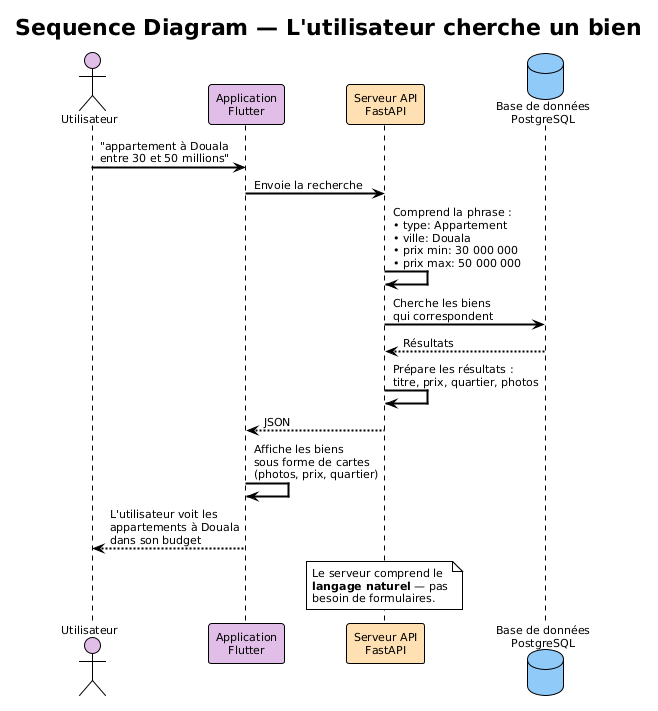
\includegraphics[width=0.9\textwidth]{Sequence Recherche.png}
    \caption{S\'equence de recherche d'un bien}
    \label{fig:annexe_sequence_recherche}
\end{figure}

\begin{figure}[H]
    \centering
    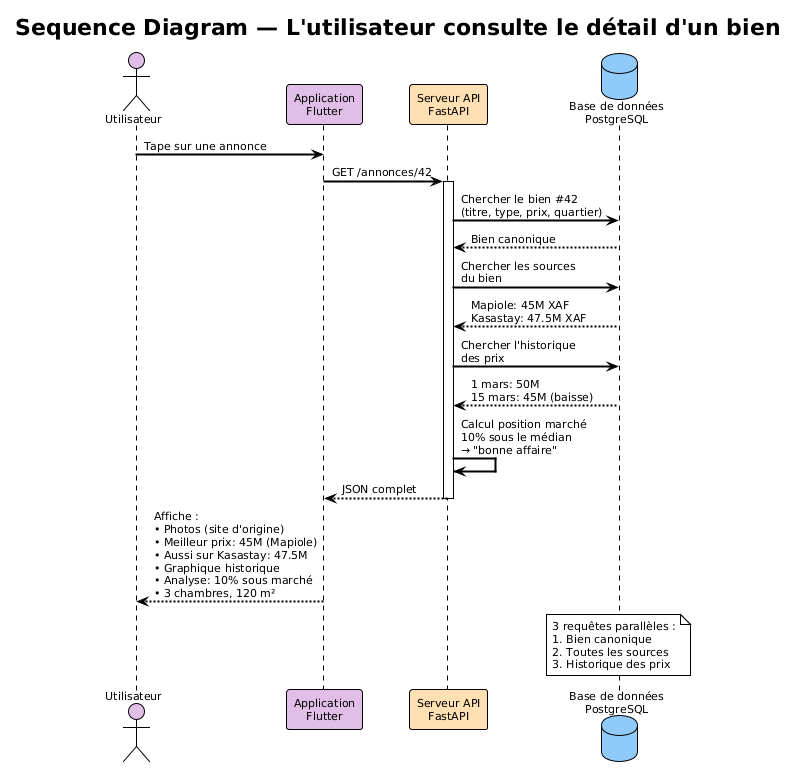
\includegraphics[width=0.9\textwidth]{Sequence Detail Bien.png}
    \caption{S\'equence de consultation du d\'etail d'un bien}
    \label{fig:annexe_sequence_detail}
\end{figure}

% ═══════════════════════════════════════════════════════════════
%  ANNEXE C — Endpoints de l'API REST
% ═══════════════════════════════════════════════════════════════

\chapter*{Annexe C --- Endpoints de l'API REST}
\addcontentsline{toc}{chapter}{Annexe C --- Endpoints de l'API REST}
\label{annexe:api}

L'API REST expos\'ee par le back-end FastAPI est organis\'ee en routeurs th\'ematiques. Le tableau ci-dessous recense les principaux endpoints consomm\'es par l'application mobile et web.

\begin{table}[H]
    \centering
    \footnotesize
    \renewcommand{\arraystretch}{1.25}
    \begin{tabularx}{\textwidth}{|l|l|X|}
        \hline
        \rowcolor{headergray}
        \textbf{M\'ethode} & \textbf{Chemin} & \textbf{Description} \\ \hline
        GET  & \texttt{/health} & Sonde de vie du serveur (statut DB, scheduler). \\ \hline
        GET  & \texttt{/annonces} & Liste pagin\'ee des fiches canoniques (filtrable par type, prix, surface, chambres). \\ \hline
        GET  & \texttt{/annonces/nearby} & Fiches canoniques proches d'un point (lat, lng, rayon). \\ \hline
        GET  & \texttt{/annonces/\{id\}} & D\'etail consolid\'e d'une fiche canonique (sources li\'ees, prix compar\'es). \\ \hline
        GET  & \texttt{/annonces/\{id\}/history} & Historique des \'ev\'enements (prix, disponibilit\'e) d'une annonce. \\ \hline
        GET  & \texttt{/annonces/\{id\}/similar} & Fiches canoniques similaires (m\^eme type, m\^eme quartier). \\ \hline
        GET  & \texttt{/annonces/\{id\}/analyse} & Analyse de positionnement de prix vs quartiers comparables. \\ \hline
        GET  & \texttt{/search} & Recherche en langage naturel (parse la requ\^ete c\^ot\'e serveur). \\ \hline
        GET  & \texttt{/search/ai} & Variante assist\'ee par IA de la recherche naturelle. \\ \hline
        POST & \texttt{/chat} & Assistant conversationnel (questions sur le march\'e). \\ \hline
        GET  & \texttt{/neighborhoods} & Liste des localisations connues (villes + quartiers). \\ \hline
        GET  & \texttt{/neighborhoods/\{slug\}} & Indicateurs d'un quartier (prix m\'edian, dur\'ee de publication, score d'activit\'e). \\ \hline
        GET  & \texttt{/neighborhoods/city/\{city\}} & Indicateurs agr\'eg\'es par ville. \\ \hline
        GET  & \texttt{/neighborhoods/trending/list} & Quartiers en croissance (tendance 90 jours). \\ \hline
        GET  & \texttt{/profiles/cities} & Profils de ville complets (price\_tier, growth, demand). \\ \hline
        GET  & \texttt{/profiles/neighborhoods/by-location/\{id\}} & Profil complet d'un quartier. \\ \hline
        GET  & \texttt{/admin/review/pending} & Annonces en attente de validation humaine (adaptateur universel). \\ \hline
        POST & \texttt{/admin/review/\{raw\_id\}} & Approuver ou refuser une annonce en attente. \\ \hline
        GET  & \texttt{/admin/sources} & Liste des sources configur\'ees. \\ \hline
        POST & \texttt{/admin/sources} & Ajouter une nouvelle source (slug, URL, type d'adaptateur). \\ \hline
        POST & \texttt{/admin/sources/\{slug\}/crawl} & D\'eclencher manuellement une collecte pour une source. \\ \hline
        POST & \texttt{/admin/analytics/recompute} & Recalculer les scores de quartiers \`a la demande. \\ \hline
        GET  & \texttt{/admin/jobs} & \'Etat des t\^aches programm\'ees (APScheduler). \\ \hline
        POST & \texttt{/payments/upgrade} & Souscription \`a un plan payant (int\'egration Mobile Money). \\ \hline
        GET  & \texttt{/payments/\{ref\}/status} & Statut d'une transaction. \\ \hline
    \end{tabularx}
    \caption{Principaux endpoints de l'API CentralImmo}
    \label{tab:api_endpoints}
\end{table}

% ═══════════════════════════════════════════════════════════════
%  ANNEXE D — Extraits du code source
% ═══════════════════════════════════════════════════════════════

\chapter*{Annexe D --- Extraits du code source}
\addcontentsline{toc}{chapter}{Annexe D --- Extraits du code source}
\label{annexe:code}

\section*{D.1 --- Algorithme de d\'eduplication (DCS)}

Calcul du Duplicate Confidence Score entre une annonce brute et une fiche canonique (\texttt{core/matcher.py}).

\begin{lstlisting}[language=Python, caption={Calcul du DCS --- \texttt{compute\_dcs}}, label={lst:dcs}]
def compute_dcs(draft, canonical, draft_location_id=None):
    f = MatchFactors(
        title_sim=_title_sim(draft.title_raw, canonical.title_canonical),
        price_proximity=_price_proximity(
            draft.price_parsed, canonical.current_best_price),
        type_match=1.0 if (draft.property_type_raw or "").lower()
            == (canonical.property_type or "").lower() else 0.0,
        surface_match=_surface_match(draft.area_sqm, canonical.area_sqm),
        bedrooms_match=_exact_or_neutral(draft.bedrooms, canonical.bedrooms),
        location_sim=_location_sim(draft_location_id,
            canonical.location_id, draft.location_raw, None),
        image_overlap=_image_overlap(draft.images_raw or [], []),
    )
    dcs = (
        0.30 * f.title_sim
        + 0.20 * f.price_proximity
        + 0.15 * f.type_match
        + 0.15 * f.surface_match
        + 0.10 * f.bedrooms_match
        + 0.05 * f.location_sim
        + 0.05 * f.image_overlap
    )
    return dcs, f
\end{lstlisting}

\section*{D.2 --- Idempotence du pipeline d'ingest}

\`A chaque collecte, le robot calcule un \texttt{url\_hash} (sha256 de l'URL normalis\'ee). S'il existe d\'ej\`a, l'annonce n'est pas r\'eins\'er\'ee : on met \`a jour sa date de collecte et on enregistre un \'ev\'enement d'historique uniquement si le prix ou la disponibilit\'e ont chang\'e (\texttt{core/ingest.py}).

\begin{lstlisting}[language=Python, caption={Boucle d'ingest idempotente}, label={lst:ingest}]
def ingest(db, drafts, source_id, crawl_session_id, adapter_kind="dedicated"):
    for draft in drafts:
        url_hash = hashlib.sha256(
            normalize_url(draft.url_source).encode("utf-8")).hexdigest()
        existing = db.query(RawListing).filter(
            RawListing.url_hash == url_hash).first()
        if existing:
            # RE-CRAWL: ne pas re-inserer, juste comparer a l'historique
            existing.crawl_session_id = crawl_session_id
            existing.crawled_at = datetime.now(timezone.utc)
            if existing.canonical_property_id:
                append_history_if_changed(db, existing.id,
                    existing.canonical_property_id, draft.price_parsed,
                    "available", crawl_session_id)
            continue
        # NOUVELLE annonce : resolution de localisation + match canonique
        location_id = resolve_location(db, draft.location_raw)
        match_result = find_canonical_match(db, draft, location_id)
        # ... insertion du RawListing + lien/creation du CanonicalProperty ...
\end{lstlisting}

\section*{D.3 --- Normalisation d'une annonce Ny\`e Ta Piole}

Le m\'ecanisme de conversion d'un JSON brut de l'API Ny\`e Ta Piole vers le format unifi\'e \texttt{RawListingDraft} (\texttt{scrapers/nyetapiole.py}). Les champs \texttt{surface}, \texttt{bedrooms} et coordonn\'ees \`a \texttt{0} sont convertis en \texttt{None} pour \'eviter de polluer la fiche canonique avec des donn\'ees absentes.

\begin{lstlisting}[language=Python, caption={Normalisation Ny\`e Ta Piole --- extrait}, label={lst:nyetapiole}]
def normalize_data(self, raw):
    slug = raw.get("slug")
    title = raw.get("title", "").strip()
    if not slug or not title:
        return None
    price = raw.get("price")
    price_parsed = int(price) if isinstance(price, (int, float)) and price > 0 else None
    district = raw.get("district") or {}
    city_name = (district.get("city") or {}).get("name", "")
    district_name = district.get("name", "")
    location_raw = f"{district_name}, {city_name}" if district_name and city_name else (city_name or district_name)
    lat = raw.get("latitude")
    lng = raw.get("longitude")
    latitude = float(lat) if isinstance(lat, (int, float)) and lat != 0 else None
    longitude = float(lng) if isinstance(lng, (int, float)) and lng != 0 else None
    bedrooms = raw.get("bedrooms")
    bedrooms = bedrooms if isinstance(bedrooms, int) and bedrooms > 0 else None
    surface = raw.get("surface")
    area_sqm = float(surface) if isinstance(surface, (int, float)) and surface > 0 else None
    return RawListingDraft(
        url_source=f"https://nyetapiole.com/property/{slug}",
        title_raw=title, price_parsed=price_parsed, currency="XAF",
        location_raw=location_raw, bedrooms=bedrooms, area_sqm=area_sqm,
        latitude=latitude, longitude=longitude, confidence=1.0,
    )
\end{lstlisting}